\section{System Architecture and Data Engineering}
\label{sec:data_acquisition}
This section details the engineering strategy adopted for the ingestion and management of the SHARAD radar data.
Given the massive scale of the available dataset and the specific scientific requirements of the project, a hybrid approach combining automated bulk ingestion with expert-supervised selection was implemented.
The pipeline is designed to ensure both efficiency in data retrieval and high geological quality in the training set.

\subsection{High-Level Pipeline Overview}
The data capabilities of the framework were organized into a sequential engineering pipeline designed to transform raw unstructured data into optimized tensor batches for deep learning.
As illustrated in Figure~\ref{fig:system_architecture2}, the workflow is highly modular and consists of four distinct operational blocks:

\begin{enumerate}
    \item \textbf{Data Acquisition \& Ingestion (Block 1):} Driven by a standardized manifest file (\texttt{url\_list.txt}), a dedicated Bash script (\texttt{auto\_wget.sh}) automatically fetches raw radar products (TIFF/IMG format) from the NASA PDS nodes.
    \item \textbf{Pre-processing \& Caching (Block 2):} Handled primarily by the \texttt{process.py} script within the \texttt{MapDataset} module. This stage performs surface alignment, horizon tracking, spatial tiling (patching), and logarithmic/MinMax normalization. The refined data is then serialized into persistent binary cache chunks.
    \item \textbf{CycleGAN Training Loop (Block 3):} A custom PyTorch DataLoader serves the cached chunks into a Docker-isolated GPU environment. Here, the dual-generator setup ($G$ for Sim$\rightarrow$Real and $F$ for Real$\rightarrow$Sim) and discriminators are optimized via cycle-consistency and adversarial losses.
    \item \textbf{Anomaly Detection Application (Block 4):} For inference, the trained Generator $G$ processes simulated inputs to create a clutter-only background reference. A difference map is computed against the real observation, which undergoes Z-score thresholding to produce the final anomaly mask.
\end{enumerate}

\begin{figure}[htbp]
    \centering
    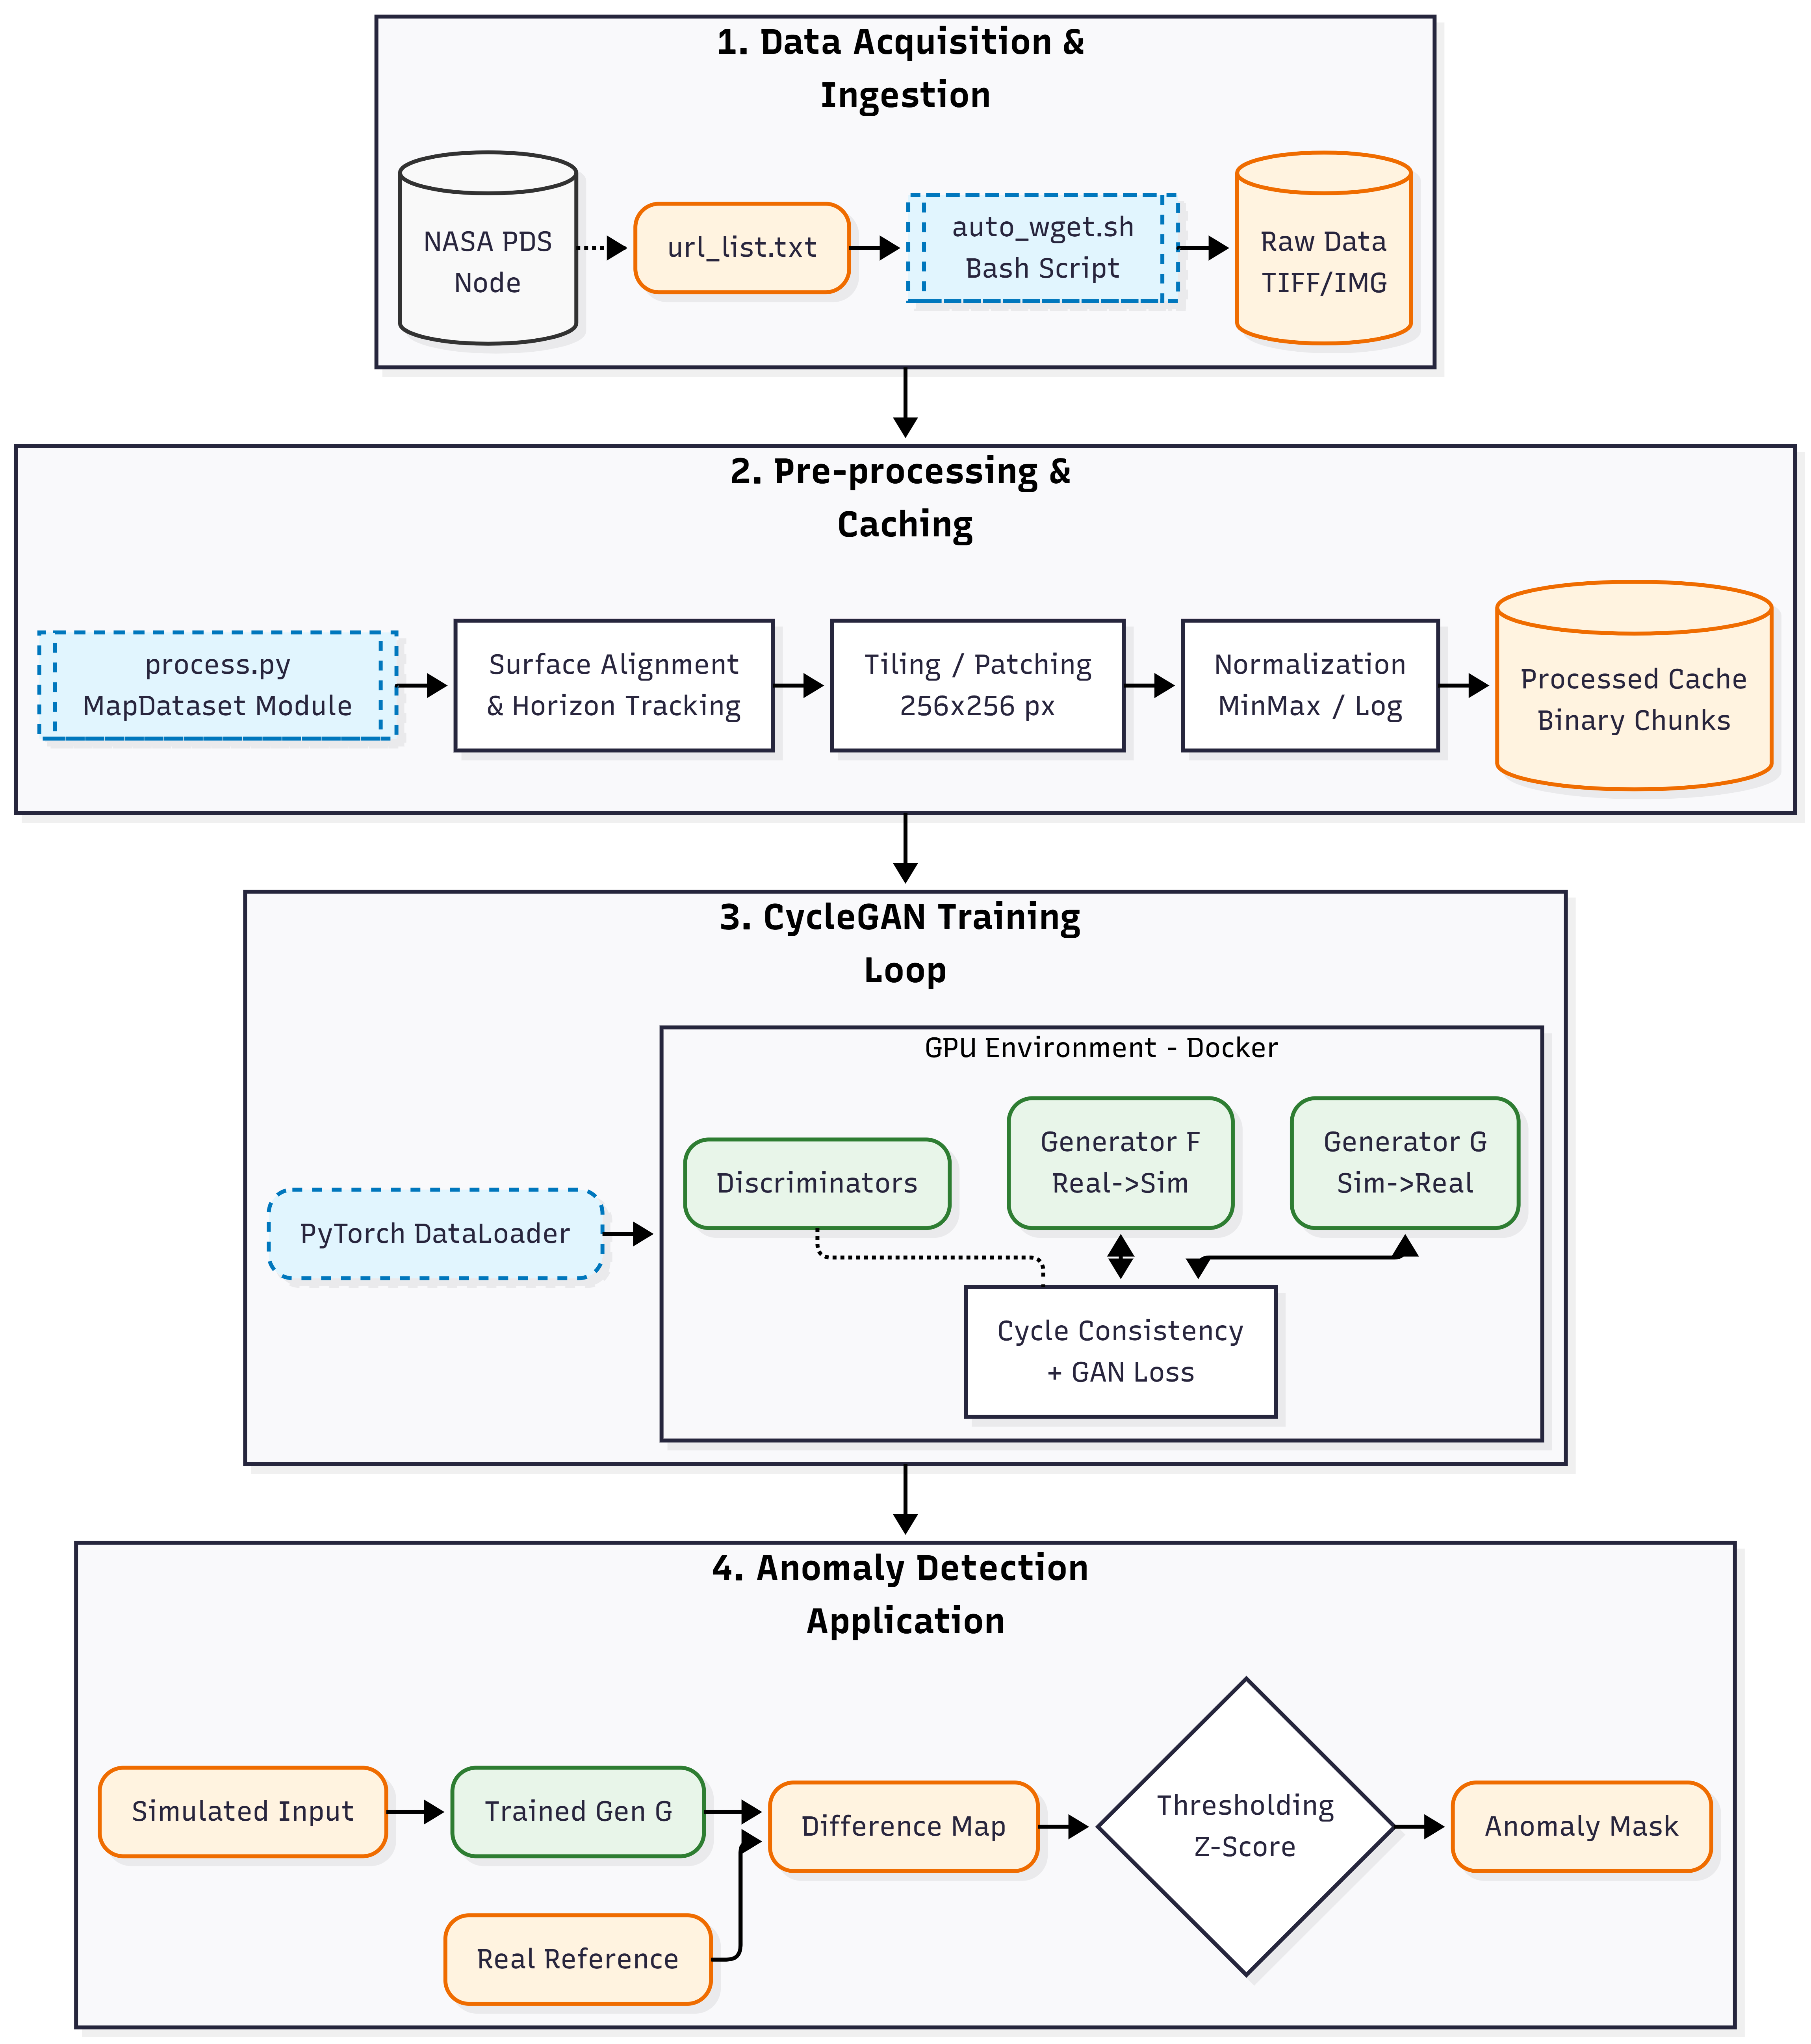
\includegraphics[width=\textwidth]{images/diagrams/high-level-system-architecture-V}
    \caption{High-level overview of the proposed system architecture. The pipeline encompasses automated data ingestion from NASA PDS (Block 1), pre-processing and efficient caching (Block 2), the CycleGAN training loop (Block 3), and the final anomaly detection application (Block 4).}
    \label{fig:system_architecture2}
\end{figure}

This modular architecture ensures that the computation-heavy pre-processing steps are decoupled from the training phase, allowing for rapid experimentation cycles once the cache is generated.

\subsection{Automated Data Acquisition}
To process the planetary-scale volume of SHARAD observations, manual data retrieval is structurally inadequate.
Consequently, a fully automated and parallelized acquisition pipeline was developed to interface directly with the NASA Planetary Data System (PDS) archives (see Block 1 of Figure~\ref{fig:system_architecture2}), which host the calibrated SHARAD radargrams and associated metadata for MRO~\cite{Zurek_2007,Seu_2007}.

The acquisition protocol is driven by a standardized manifest file (\texttt{url\_list.txt}) containing the Universal Resource Identifiers (URIs) of the target observations, ensuring complete experimental reproducibility.
To optimize the retrieval phase, the pipeline employs a concurrent fetching strategy (orchestrated via \texttt{auto\_wget.sh}) that maximizes network bandwidth utilization, drastically reducing the dataset initialization time. 

Given the massive scale of the data (often spanning hundreds of gigabytes) and the potential for network instability, the ingestion system is designed with strict fault-tolerance mechanisms.
It incorporates state-tracking to verify local data integrity prior to initiating transfers, thereby avoiding redundant downloads and allowing the ingestion process to be safely interrupted and resumed.
This robust data engineering foundation is essential to guarantee that the subsequent deep learning models are trained on a complete, uncorrupted representation of the target geological regions~\cite{yebasse2025advances}.

\subsection{Region of Interest (ROI) Selection: A Hybrid Strategy}
While the ingestion of raw data is fully automated, the specific selection of data segments for training and testing---the Regions of Interest (ROI)---followed a nuanced strategy that balances the massive data requirements of deep learning with the need for rigorous scientific evaluation.
This decision represents a deliberate trade-off between engineering automation, dataset size, and the \enquote{cleanliness} of the data distribution, as discussed in the context of SHARAD-based geological studies in~\cite{foss2017sharad3d,yebasse2025advances}.

